\chapter{Data Centre Introduction}

\section{IT equipment}

The data centre exists to house IT equipment.
Broadly, this can be broken down into:
\begin{description}
\item[Servers] providing compute capability. May be single-purpose servers, virtualisation hosts, modular multiple-unit blade server enclosures or larger mainframe equipment.
\item[Storage systems] providing aggregate storage to servers, such as dedicated NAS and SAN devices. May also include backup-centric storage such as tape storage systems.
\item[Networking equipment] including switches (unmanaged, L2/L3 managed), routers, hardware firewalls, hardware VPN, WAN termination and routing equipment.
\item[Management equipment] including local KVM, remote KVM, KVM-over-IP, serial console servers, smart power distribution units.
\end{description}


\section{Data hall}

The data hall is the main area of interest in a data centre where IT equipment is housed, \autoref{fig:data-hall-schematic}.
Data centre environments may have one or more data halls, sometimes called suites.

\begin{figure}[htbp]
  \centering
  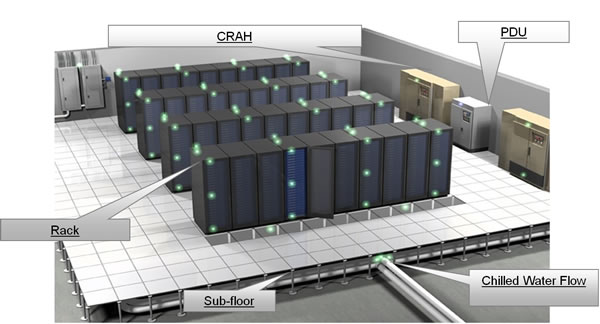
\includegraphics[width=1.0\linewidth]{data_hall}
  \caption{Data hall schematic (TSM tutorials)}
  \label{fig:data-hall-schematic}
\end{figure}

\subsection{Raised floor}

The data hall often has a raised floor, meaning that the tiles can be removed and a space exists under the floor, \autoref{fig:raised-floor}.
It is somewhat similar to a false-ceiling in reverse.

\begin{figure}[htbp]
  \centering
  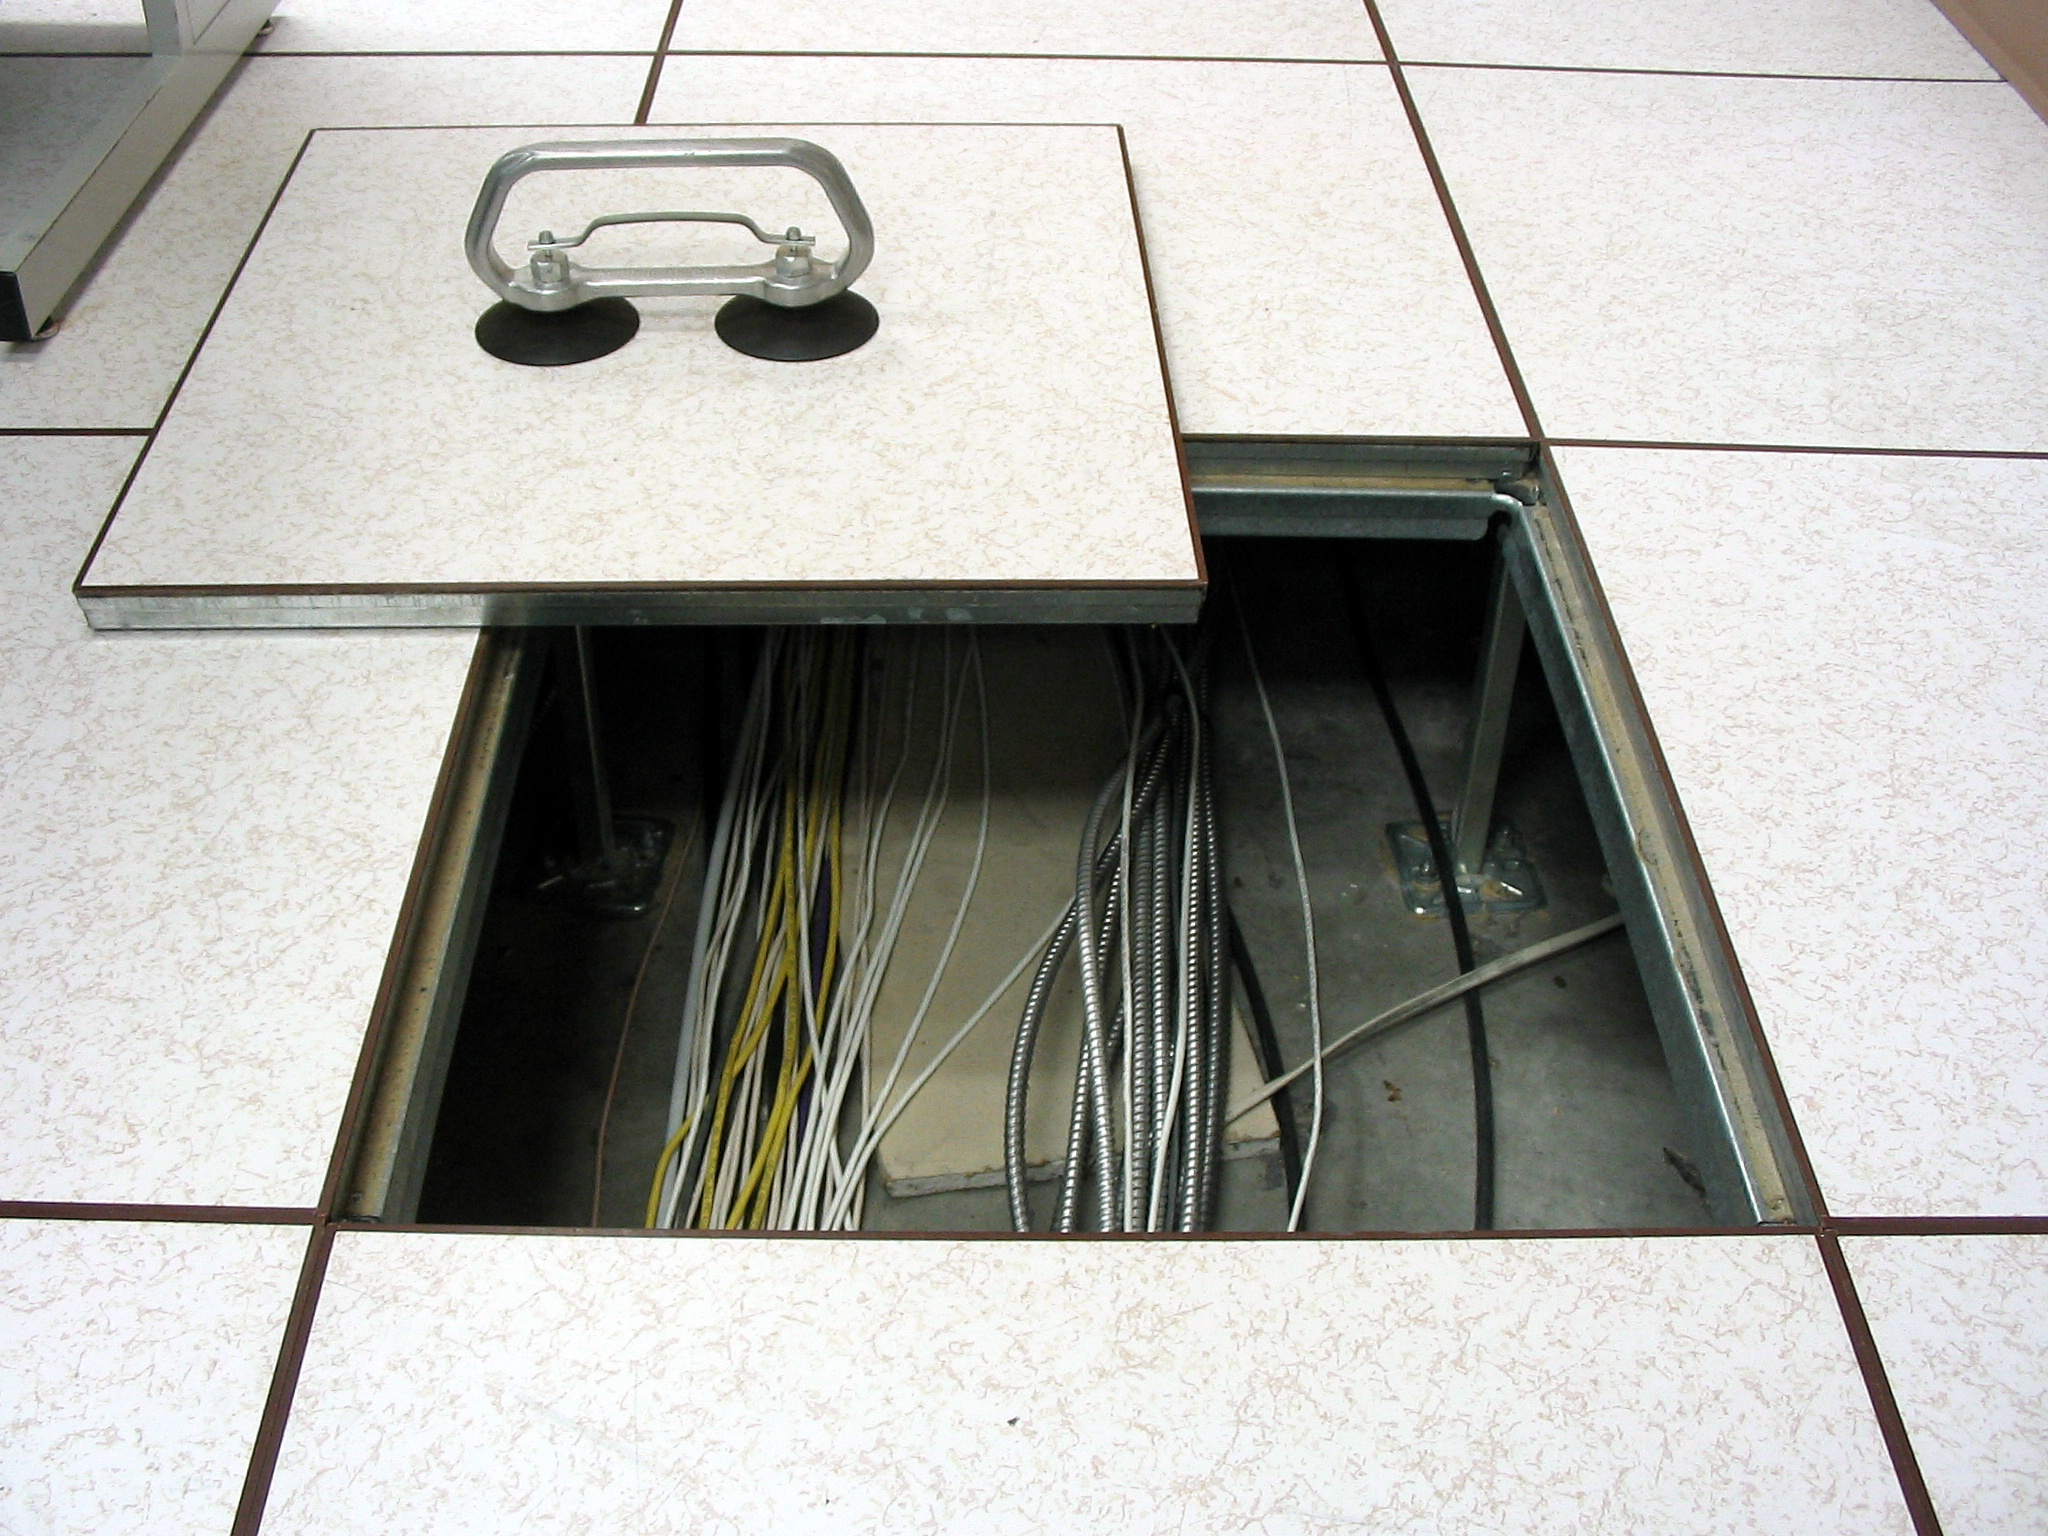
\includegraphics[width=0.75\linewidth]{raised_floor_wikipedia}
  \caption{Raised floor (Wikipedia)}
  \label{fig:raised-floor}
\end{figure}

Not all data centres have raised floors.
Where present, the raised floor has two key functions:
\begin{itemize}
\item Provides space for cooling air to circulate. Some times are solid but others are perforated to allow air to escape. More on that later.
\item Allows cables to be routed and re-routed easily. 
\end{itemize}

\subsection{Infrastructural equipment}

All data halls will vary.
However, most will include some/all of the following:
\begin{description}
\item[Power distribution] panels including circuit breakers, switches and meters. Also may include floor-standing UPS units.
\item[Climate control] equipment to maintain the room temperature and humidity in allowable ranges, often termed CRAC or CRAH.
\item[Fire] detection and suppression equipment.
\item[Security] equipment including access control devices, motion sensing and video cameras.
\end{description}

\subsection{Cage}

A cage is a subdivision of a data hall to demarcate a number of racks for security or regulatory purposes.

\begin{figure}[htbp]
  \centering
  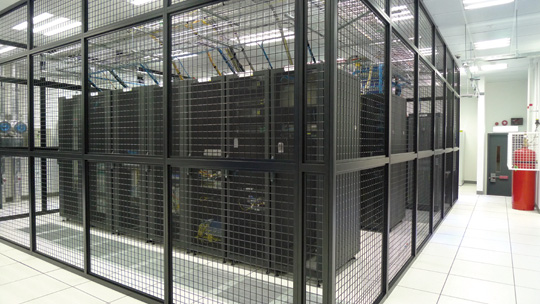
\includegraphics[width=1.0\linewidth]{cage}
  \caption{Cage (Equinix)}
  \label{fig:cage}
\end{figure}


\section{Form factor}

\subsection{Rack units}

IT equipment in data centre environments is normally rack-mount form.
Rack-mount equipment has a standard width of \SI{48.3}{\centi\metre} or 19~inches, which includes the rack ears protruding from the side of each piece of equipment.

Equipment height is standardised in multiples of \SI{44.5}{\milli\metre} or 1.752~inches.
One rack unit (commonly called 1U) is equivalent to \SI{44.5}{\milli\metre}.
Conventionally we just use the number of units, such as 4U.

\subsection{Blade servers}

You will sometimes encounter so-called Blade Servers in high-performance computing environments.
A blade system consists of a chassis that holds a number of individual blade servers, \autoref{fig:blade-server-enclosure}.
Each blade server is a fully functional server but is powered and may receive connectivity via a backplane in the enclosure.
Blade servers needs to be managed carefully as their power density is very high.
\begin{figure}[htbp]
  \centering
  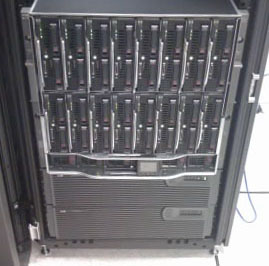
\includegraphics[width=0.3\linewidth]{blade_server_enclosure}
  \caption{Blade server enclosure (Wikipedia)}
  \label{fig:blade-server-enclosure}
\end{figure}

\subsection{Non-rackmount equipment}

Non-rackmount equipment such as tower-type server PCs should be discouraged in data centre environments.
Sometimes legacy equipment has to be accomodated.
The only exception to this would be large equipment like mainframe computers which are supplied in a cabinet case, \autoref{fig:ibm-mainframe}.

\begin{figure}[htbp]
  \centering
  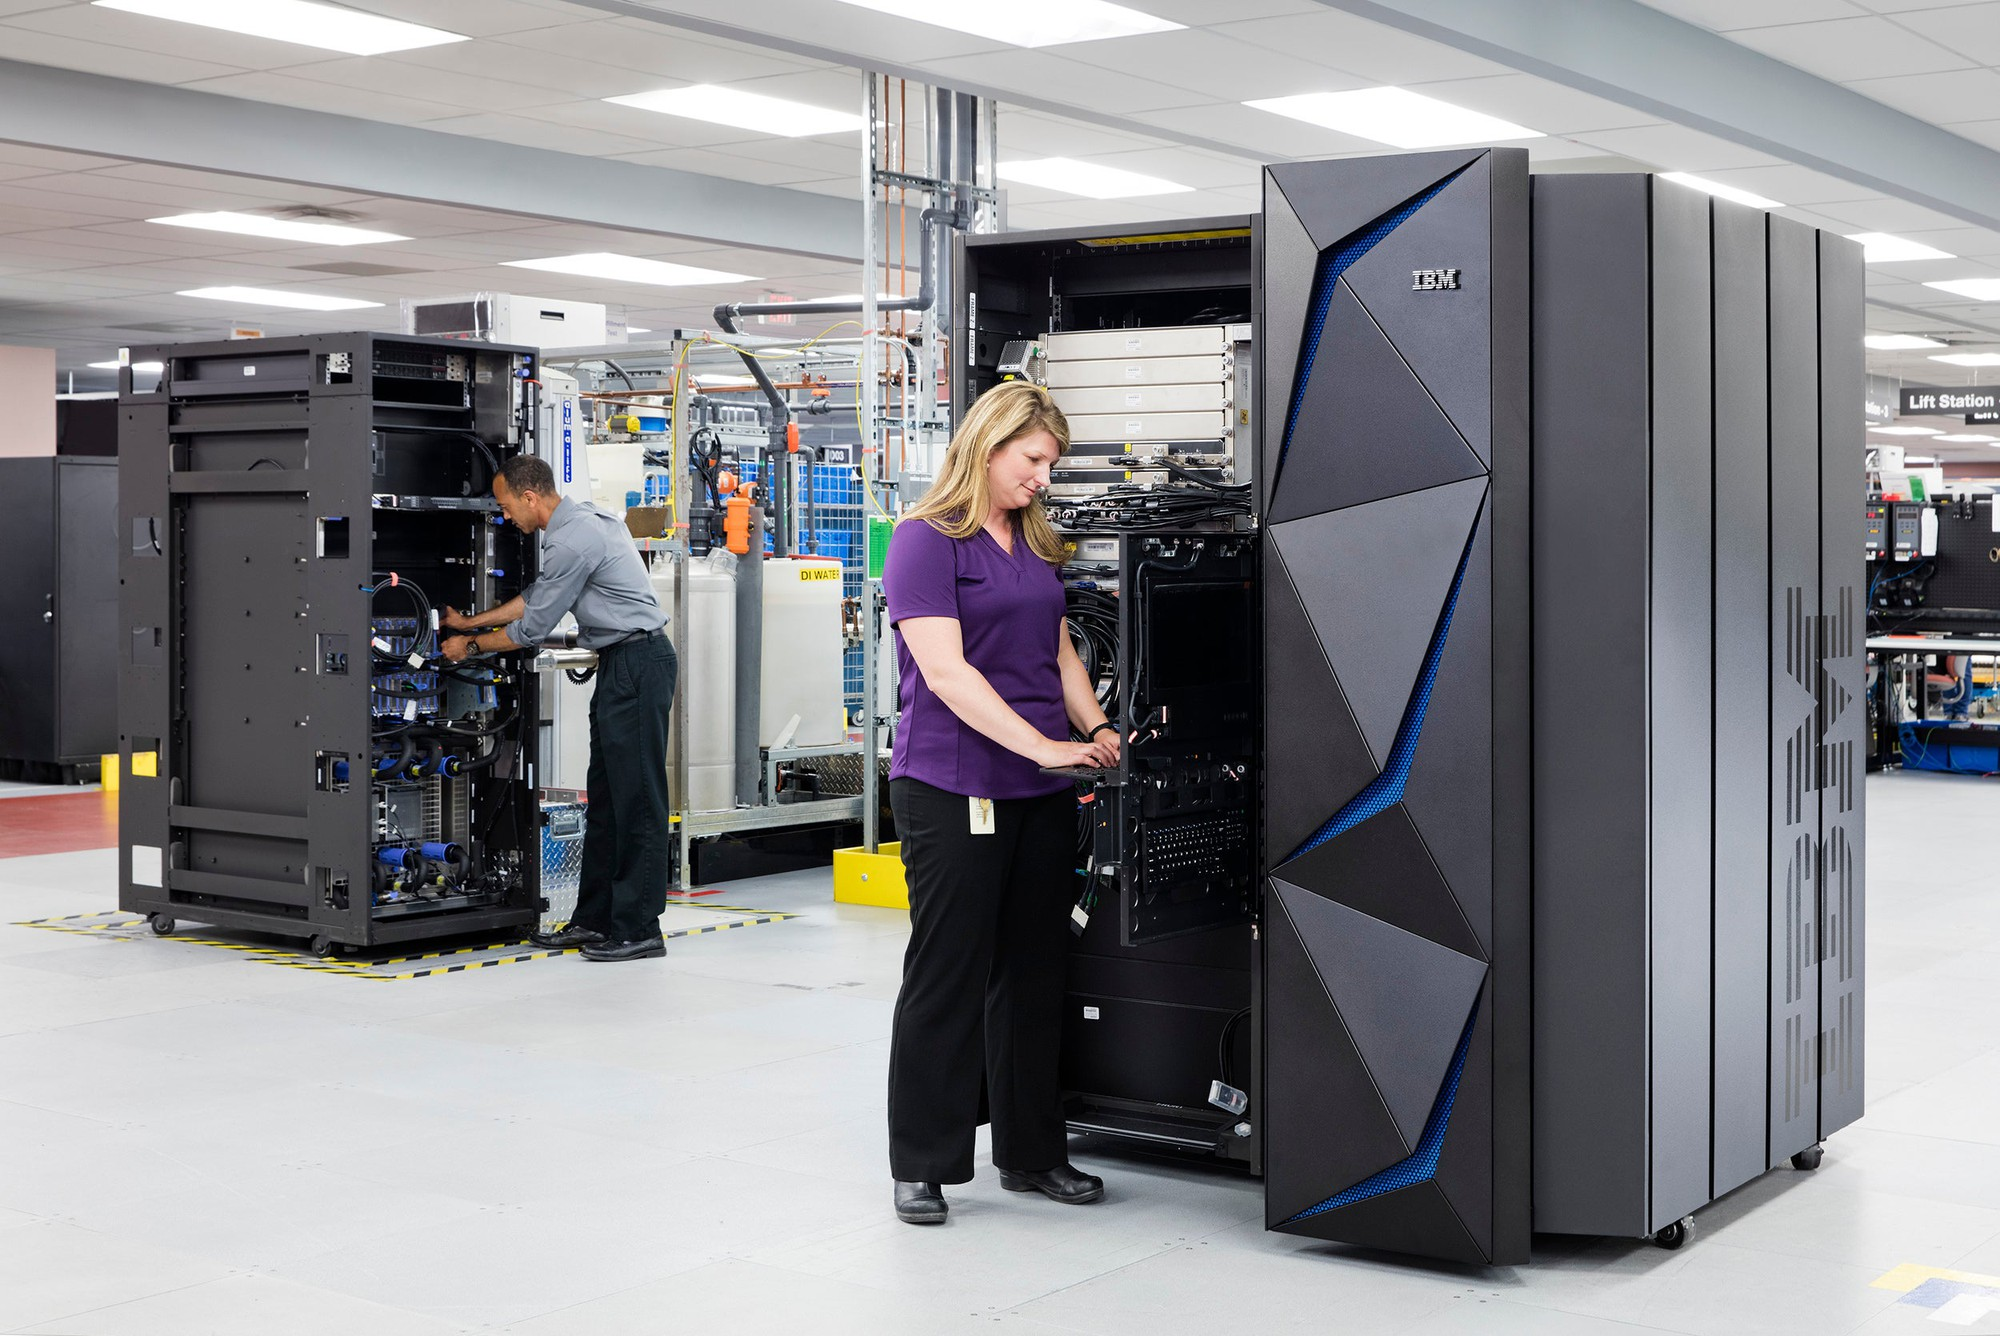
\includegraphics[width=0.5\linewidth]{ibm_mainframe}
  \caption{IBM mainframe}
  \label{fig:ibm-mainframe}
\end{figure}


\section{Equipment layout}

IT equipment is mounted in racks within cabinets.
Cabinets make up rows and pairs of rows make up aisles.


\subsection{Cabinet}

A cabinet contains front-and-back vertical rack rails, and is secured by a lockable door, usually perforated.
Equipment is racked within the cabinet.
Standard full-size cabinets are 42U in height, with each position numbered from the bottom upwards.

\begin{figure*}[htbp]
  \centering
  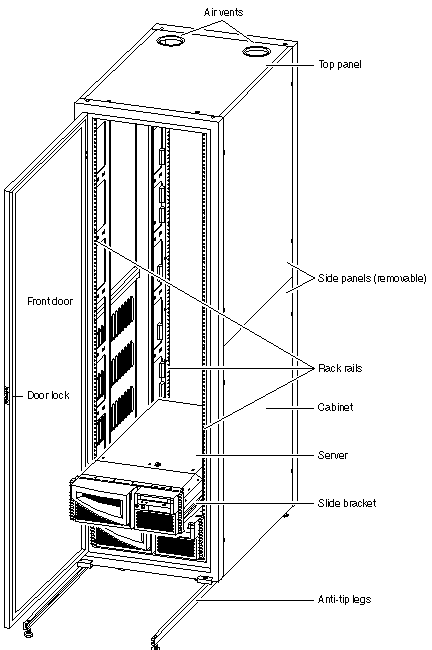
\includegraphics[width=1.0\linewidth,height=0.8\paperheight,keepaspectratio]{cabinet}
  \caption{19-inch cabinet schematic (Oracle)}
  \label{fig:cabinet}
\end{figure*}

Most servers, like desktop computers, are air cooled.
Air is drawn in at the front and ejected out the rear of the server.
Servers are always racked front-to-back.

\begin{figure}[htbp]
  \centering
  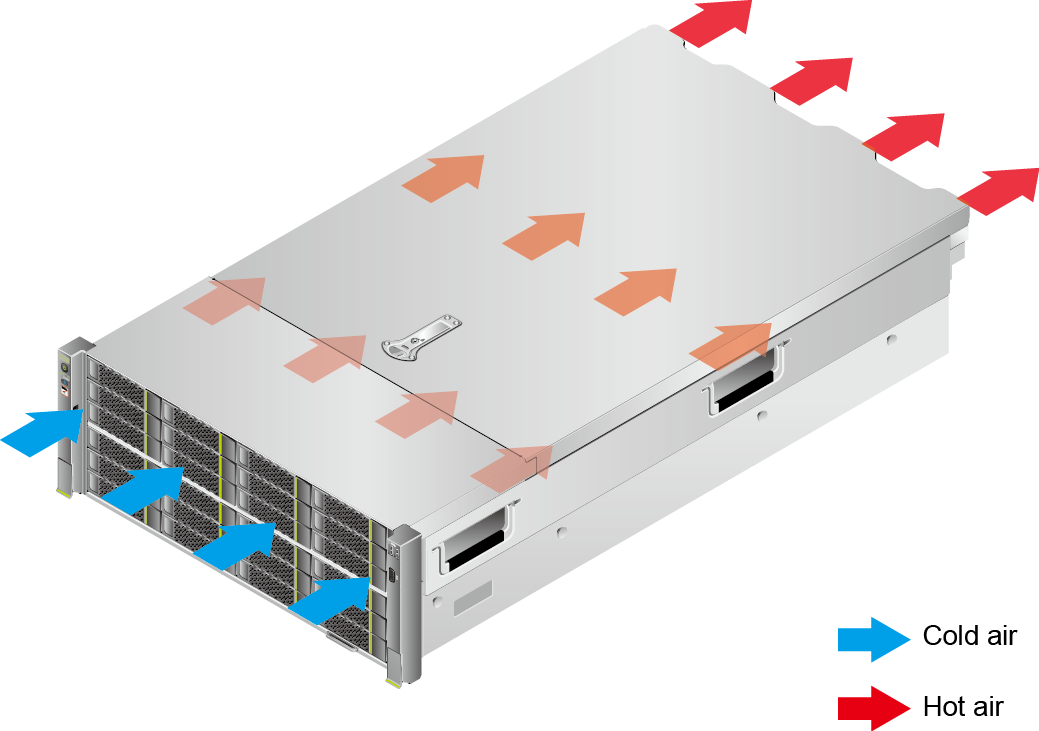
\includegraphics[1.0\linewidth]{server_airflow_huawei}
  \caption{Conventional front-to-back server airflow}
  \label{fig:server-airflow}
\end{figure}

Cabling is normally done at the rear of the rack.
Networking and power distribution equipment is often (but not always) mounted at the rear of a cabinet facing the rear.


\subsection{Rack mounting}

Racks have holes drilled in them for allowing equipment to be secured.
These are normally unthreaded, and allow cage nuts and bolts to be inserted.
The cage nut inserts into the rack, whilst the bolt is inserted through the holes drilled in the IT equipment's rack ears.

\begin{figure}[htbp]
  \centering
  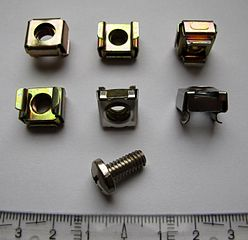
\includegraphics[width=0.75\linewidth]{cage_nut}
  \caption{Cage nuts and bolt (wikipedia)}
  \label{fig:cage-nut}
\end{figure}

Heavier pieces of equipment such as servers normally are placed on horizontal rails inserted into the rack first.
The rails are secured to the front and back racks.

\subsection{Rows}

Where more than one cabinet is required, they are normally placed beside each other to form a row.
The number of cabinets in a row will depend on spatial and usage requirements.

\subsection{Aisle}

An aisle is where two rows of cabinets face each other.
Data centres normally use a hot aisle/cold aisle arrangement where servers face each other front-on or rear-on.
This is to aid in cooling (see later).

\begin{figure}[htbp]
  \centering
  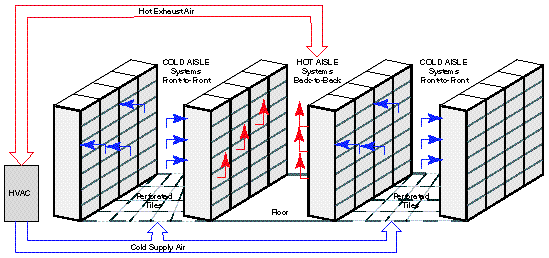
\includegraphics[width=1.0\linewidth]{hot_cold_aisle_oracle}
  \caption{Hot/cold aisle (Oracle)}
  \label{fig:hot-cold-aisle}
\end{figure}



\section{Regulation}

\begin{description}
\item[Reliability standards] govern to what degree a data centre can be described as fault-tolerent:
  \begin{description}
  \item[Uptime institute] has a number of ``tiers'' which summarise how reliable a particular data centre environment is.
  \item[TIA-942] has a number of similar tiers that are primarily dependent on reliability and redundancy
  \end{description}
\item[Efficiency standards] aim to minimise the energy usage and environmental impact of data centres:
\begin{description}
\item[LEED]
\end{description}
\item[Data-related legislation] has legal effect and may have ramifications in certain data centre environments:
  \begin{description}
  \item[GDPR] governing personal data
  \item[FOI] ensuring right of access to own personal data and to aggregate public data. Similar FOI laws exist in many countries.
  \item[HIPPA] controlling how health data is stored and process
  \item[COPPA] controlling how personal data of children is used and collected, including how consent from children/parents is taken for data processing.
  \end{description}
\item[Industry standards] often are a requirement to do business in certain sectors and need to be followed:
  \begin{description}
  \item[PCI/DSS] relating to handling and storage of payment card data. Compliance is normally a condition of being given merchant facilities.
  \item[ISO 27001] relating to storage/handling of general data in a secure fashion.  Compliance is often a condition of being awarded business from certain public and private organisations.
  \end{description}
\end{description}


\subsection{Key trends}

There are a number of trends globally that are influencing data centre design and usage:
\begin{description}
\item[Virtualisation] is becoming much more common where a hypervisor manages multiple operating systems on a single physical machine. 
\item[Cloud] is a greater focus.  Both in terms of replacement of certain on-site infrastructure with cloud services, integration in a hybrid onsite/cloud setup and provision of private cloud facilities.
\item[Security] is now a main focus area, and generally needs to be handled throughout all other activities as standard practice.
\item[Environmental awareness] both for energy saving, cost reduction and business reputation. 
\item[Automation] to reduce the need for physical visits to the data centre environment.
\end{description}

\begin{figure}[htbp]
  \centering
  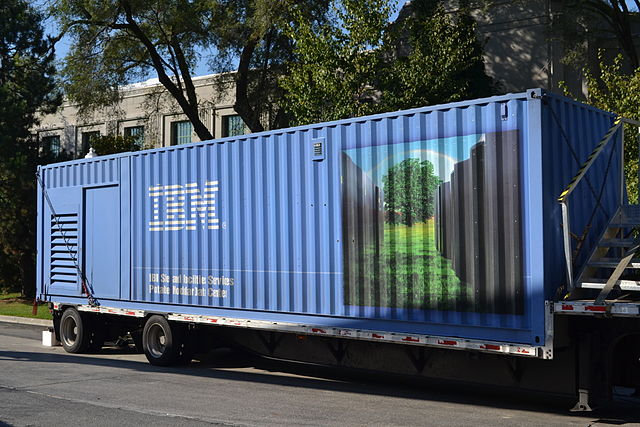
\includegraphics[width=1.0\linewidth]{modular_data_centre}
  \caption{Modular data centre (IBM/Wikipedia)}
  \label{fig:modular-data-centre}
\end{figure}

\section{People involved}

\begin{description}
\item[Customer]
  We will use customer to mean a customer of data centre services, as opposed to end user who utilises the services provided.
  The data centre customer has essentially got two options: on-site or co-located data centre.
\item[End users]
  People / systems who use the services provided by our data centre environment.
  They normally have expectations of availability, reliability but are not connected with the running of the data centre.
\item[Estates / Facilities management personnel]
  Depending on the facilty, a demarcation between the roles of data centre and facilites management will exist.
  This will become evident in things around power, cooling and fire alarm infrastructure.
  The relationship between data centre managers / technicians and facilities management professionals is a key asset to a well-run data centre environment.
\end{description}
  
\section{On-site}

Many organisations operate some on-site data centre provision:
\begin{itemize}
\item
  Some organisations may build and operate dedicated data centres for their own use.
\item
  Many organisations will have a data centre that forms part of a larger facility, such as a hospital or college.
  It is often the case that non-IT personnel might have no idea that the facility has a data centre or where it is.
\item 
  Often, it's not even noticed or considered by the persons owning them.
  Even a NAS box stuffed in a corner that holds critical data needs to be considered as part of data centre provision!
\end{itemize}

\subsection{Connectivity}

An on-site data centre will need WAN connections to be ordered.
These may take a number of forms such as standard DSL, GPON fibre, leased lines, microwave links.
Carrier-owned equipment is often required and connects to customer owned equipment at the so-called demarcation point.

An on-site data centre located within a larger facility will also often form the central hub of the end-user-facing networking throughout the building or site, such as the office LAN.

\subsection{Responsibilities}

On-site data centres need careful co-ordination of different responsibilities:
\begin{description}
\item[IT personnel] normally undertake network admin, system admin, patching and other IT-related duties.
\item[Facilities management] normally look after plant such as heating/cooling, parts of the electrical system and may have to facilitate copper/fibre installations.
\end{description}
Where exactly the demarcation between both sets of staff occurs is fluid and organisation-dependent.
However, it is essential that the IT staff have a basic knowledge of certain mechanical and electrical concepts to facilitate productive interaction. 

\section{Co-location}

Co-location is where a customer rents space from a so-called co-location facility, or co-lo.

\subsection{Renting}

Co-los rent space in various different units:
\begin{description}
\item[Rack spaces] in single/multiple units.
\item[Full cabinet] where the customer has use of a single cabinet in its entirety and can populate it as they wish.
\item[Cage] is a restricted area within the airspace of the data hall that is for a single customer's use.  They can normally populate the cabinets within it (supplied by the data centre) as they wish. 
\item[Suite] is where an entire data hall is provided to a single customer.
\end{description}

\subsection{Networking}

Within a co-lo environment, the customer is solely responsible for their own networking.
This means that the co-lo provider \textit{does not} supply IP addresses or outbound connectivity as standard.
Customers must have the appropriate networking cables and equipment to adequately connect their own equipment together.

\subsection{Cross-connects}

Customers may sometimes have equipment in multiple cabinets, or may wish to connect directly to other data centre customers.
They can do this by ordering a cross-connect from the co-lo provider.
Depending on the provider, there may be a charge for this service.

\subsection{Carrier connection}

Most links to locations away from the data centre will be made via telecommunication carriers.

Whilst some data centres historically have restricted the carriers a customer can use, indeed many have been operated by telecommunications carriers themselves, most are said to be carrier-neutral.

Carriers normally terminate their connections in a so-called meet-me room (MMR).
The meet-me room allows patching through cross-connects to the customer's equipment in the data hall. 

It is the responsibility of the customer to order the WAN service from the carrier, and to order the appropriate cross connect from the co-lo provider.


\section{Business needs}

Business needs must drive the choice of data centre provision.
Some key questions include:
\begin{enumerate}
\item Is the workload better served by cloud or data-centre provision in the first place?
\item Are the users of the workload located in one particular site? Or are they distributed amongst multiple distinct sites or the wider internet? 
\item How criticial is the workload to on-site business continuity?
\item What volume of data is likely to be exchanged between end-users and the data centre?
\item Can your on-site services match those a co-located provider can offer? 
\end{enumerate}
The solution chosen is often a compromise, and frequently a combination of multiple modes. For example:
\begin{itemize}
\item  A supermarket chain might be best suited with a small on-site server room for in-store services, use a co-lo for central services and a cloud provision for its online store.
\end{itemize}




